\documentclass[11pt,letterpaper,boxed]{pset}

\usepackage[margin=0.75in]{geometry}
\usepackage{ulem}

\begin{document}

    \problemlist{PHYS051 HW12}
    \begin{center}
        *E41.24, E41.30, E41.40, P44.2, P44.4, SUP12.1
    \end{center}
    
    \begin{problem} [*E41.24]
        In costume jewelry, rhinestones (made of glass with $n=1.5$) are often coated with silicon monoxide ($n=2.0$) to make them more reflective. How thick should the coating be to achieve strong reflection for 560-nm light, incident normally?
    \end{problem}
    \newpage
    
    \begin{problem} [E41.30]
        An oil drop ($n = 1.20$) floats on a water ($n = 1.33$) surface and is observed from above by a reflected light (see Fig. 41-26). 
        
        \begin{enumerate}
            \item [a.] Will the outer (thinnest) regions of the drop correspond to a bright or a dark region? 
            \item [b.] How thick is the oil film where one observes the third blue region from the outside of the drop? 
            \item [c.] Why do the colors gradually disappear as the oil thickness becomes larger?
        \end{enumerate}
    \end{problem}
    
    \begin{figure} [ht]
        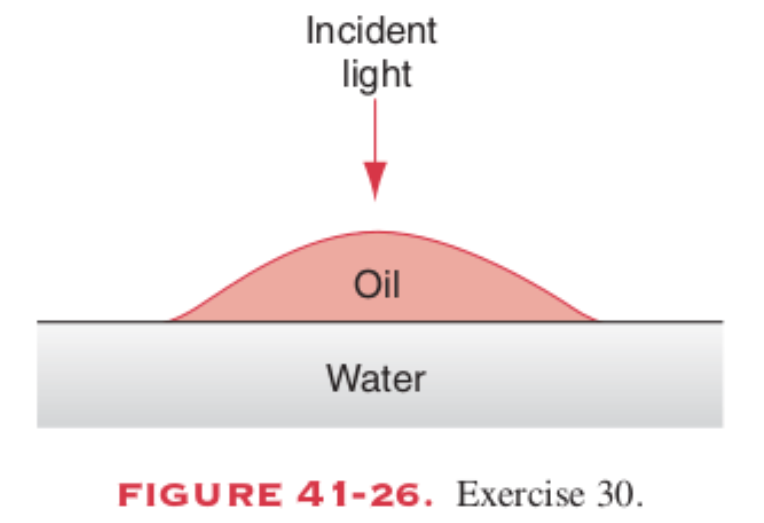
\includegraphics[width=125px]{HW12Images/E41-30.png}
    \end{figure}
    \newpage
    
    \begin{problem} [E41.40]
        An airtight chamber 5.0 cm long with glass windows is placed in one arm of a Michelson interferometer as indicated in Fig. 41-28. Light of wavelength $\lambda=500$ nm is used. The air is slowly evacuated from the chamber using a vacuum pump. While the air is being removed, 60 fringes are observed to pass through the view. From these data, find the index of refraction of air at atmospheric pressure.
    \end{problem}
    
    \begin{figure} [ht]
        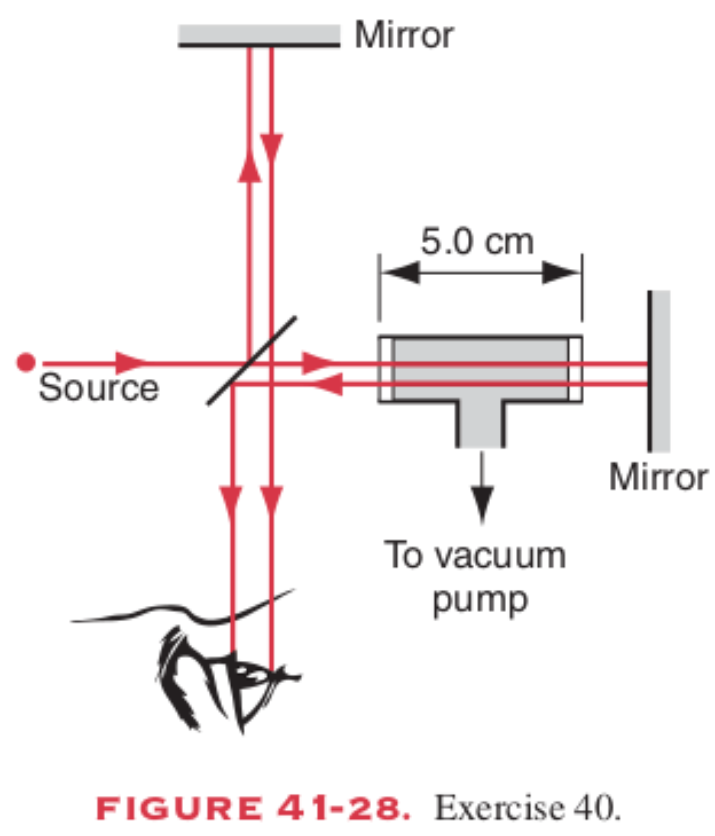
\includegraphics[width=125px]{HW12Images/E41-40.png}
    \end{figure}
    \newpage
    
    \begin{problem} [P44.2]
        A beam of light is a mixture of polarized and unpolarized light. When it is sent through a polarizing sheet, we find that the transmitted intensity can be varied by a factor of five depending on the orientation of the polarizing sheet. Find the relative intensities of these two components of the incident beam.
    \end{problem}
    \newpage
    
    \begin{problem} [P44.4]
        It is desired to rotate the plane of vibration of a beam of polarized light by $90^{\circ}$.
        
        \begin{enumerate}
            \item [a.] How might this be done using only polarizing sheets?
            \item [b.] How many sheets are required for the total intensity loss to be less than 5.0\%?
        \end{enumerate}
    \end{problem}
    \newpage
    
    \begin{problem} [SUP12.1]
        A monochromatic beam of unpolarized light with intensity $I_o$ is incident upon a series of optical elements -- polarizers, half-wave plates, and quarter-wave plates. In the figure below, the orientations of the transmission axes of the polarizers and the optic axes of the $\lambda/2$ ad $\lambda/4$ plates are given with respect to the first polarizer $P_1$.
        
        \begin{enumerate}
            \item [a.] What is the intensity after polarizer $P_1$?
            \item [b.] After $P_2$?
            \item [c.] After $P_3$?
        \end{enumerate}
    \end{problem}
    
    \begin{figure} [ht]
        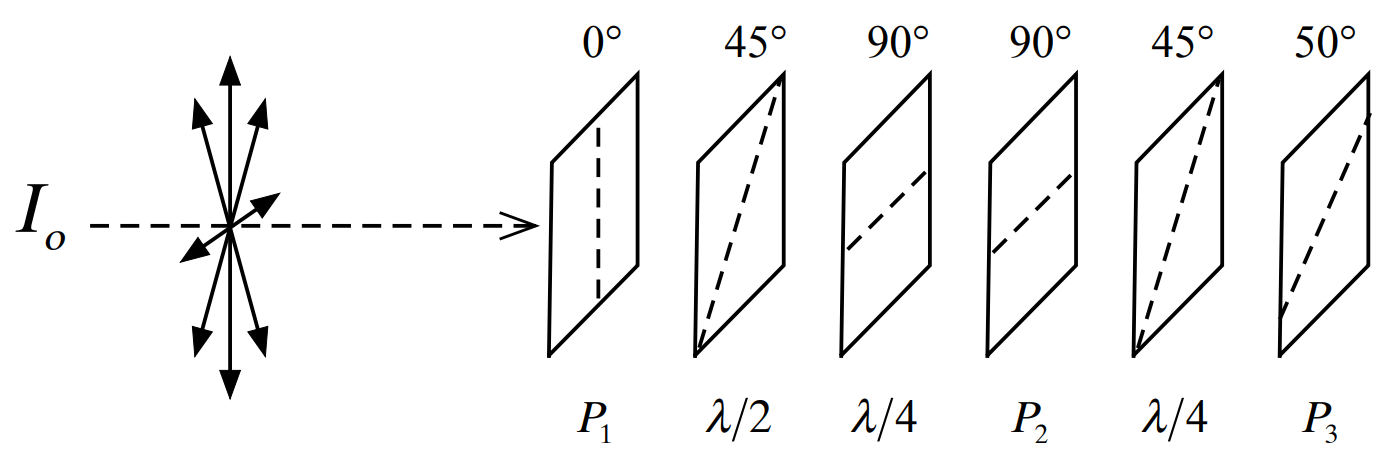
\includegraphics[width=225px]{HW12Images/SUP12-1.png}
    \end{figure}
\end{document}